\section{Parametrizations of Affine Varieties}


\begin{exercise}{1}
Parametrize all solutions of the linear equations
\begin{align*}
    x + 2y - 2z + w =& -1\\
    x + y + z - w =& 2.
\end{align*}
\end{exercise}
\begin{proof}
    By subtracting the two equations, we get
    \begin{align*}
        y - 3z + 2w = -3.
    \end{align*}
    So taking $z$ and $w$ as parameters, we get
    \begin{align*}
        y = 3z - 2w - 3
    \end{align*}
    and
    \begin{align*}
        x
        =& 2 - y - z +w\\
        =& 2 -3z +2w + 3 -z + w\\
        =& 5 - 4z + 3w.
    \end{align*}
    We get the parametrization:
    \begin{align*}
        x =& -4t + 3s + 5\\
        y =& 3t + 2s - 3\\
        z =& t\\
        w =& s.
    \end{align*}
\end{proof}

\begin{exercise}{2}
    Use a trigonometric identity to show that
    \begin{align*}
        x =& \cos(t),\\
        y =& \cos(2t)
    \end{align*}
    parametrizes a portion of a parabola. 
    Indicate exactly what portion of the parabola is covered.
\end{exercise}
\begin{proof}
    We see that for a certain $t$ that
    \begin{align*}
        y = \cos(2t) = 2\cos^2(t) - 1 = 2x^2 - 1.
    \end{align*}
    Furthermore, we know that $\cos(t)\in [-1,1]$. 
    So we know that $(\cos(t), \cos(2t))$ always lies in the portion of the parabola $y = 2x^2 -1$ where $x\in [-1,1]$.
    
    Conversely, take some $(x,y)$ with $x\in [-1,1]$ and $y = 2x^2 - 1$. 
    Then we know that there is some $t$ such that $x=\cos(t)$. 
    Then,
    \begin{align*}
        y = 2x^2 - 1 = 2\cos^2(t) - 1 = \cos(2t).
    \end{align*}
\end{proof}

\begin{exercise}{3}
Given $f\in k[x]$, find a parametrization of $\bV(y - f(x))$.
\end{exercise}
\begin{proof}
    A parametrization is clearly given by
    \begin{align*}
        x =& t\\
        y =& f(t).
    \end{align*}
\end{proof}

\begin{exercise}{4}
Consider the parametric representation
\begin{align*}
    x=\frac{t}{1+t},\,\,y=1-\frac{1}{t^2}.
\end{align*}
\begin{enumerate}
    \item Find the equation of the affine variety determined by the above parametric equations.
    \item Show that the above equations parametrize all points of the variety found in part (1) except for the point $(1,1)$.
\end{enumerate}
\end{exercise}
\begin{proof}
\begin{enumerate}
    \item We have 
    \begin{align*}
        &x = \frac{t}{1+t} &&\iff\\
        &x(1+t) = t &&\iff\\
        &x = t(1-x) &&\iff\\
        &t = \frac{x}{1-x},
    \end{align*}
    so that replacing in the equation of $y$ we obtain the equation of the affine variety
    \begin{align*}
        y =& 1 -\frac{1}{\left(\frac{x}{1-x}\right)^2}\\
        =& 1-\frac{(1-x)^2}{x^2}\\
        =& \frac{x^2-1+2x-x^2}{x^2}\iff\\
        &yx^2-2x+1=0.
    \end{align*}
    \item To show this, we simply replace the parametrised equation for $x$ and $y$ in the equation of the affine variety
    \begin{align*}
        &\parens{1-\frac{1}{t^2}}\parens{\frac{t}{1+t}}^2-2\parens{\frac{t}{1+t}}+1=0\\
        &\parens{\frac{t^2(t^2-1)}{t^2(1+t)^2}}-2\parens{\frac{t^3(1+t)}{t^2(1+t)^2}}+1=0\\
        &\parens{\frac{t^4-t^2-2t^3-2t^4}{t^2(1+t)^2}}+1=0\\
        &\frac{t^4-t^2-2t^3-2t^4+t^2(1+t)^2}{t^2(1+t)^2}=0\\
        &\frac{t^4-t^2-2t^3-2t^4+t^2(1+2t+t^2)}{t^2(1+t)^2}=0\\
        &\frac{t^4-t^2-2t^3-2t^4+t^2+2t^3+t^4)}{t^2(1+t)^2}=0\\
        &0=0.
    \end{align*}
    Notice, however, that if $x=1$, then $1=t/(1+t)$ so that $1+t=t$ which is a contradiction.
\end{enumerate}
\end{proof}

\begin{exercise}{5}
    This problem will be concerned with the hyperbola $x^2 - y^2 = 1$.
    \begin{enumerate}
        \item Just as trigonometric functions are used to parametrize the circle, hyperbolic functions are used to parametrize the hyperbola. Show that the point
        \begin{align*}
            x= & \cosh(t),\\
            y= & \sinh(t)
        \end{align*}
        always lies on $x^2 - y^2 = 1$. 
        What portion of the hyperbola is covered?
        \item Show that a straight line meets a hyperbola in $0$, $1$ or $2$ points, and illustrate your answer with a picture.
        \item Adapt the argument given at the end of the section to derive a parametrization of the hyperbola.
        \item The parametrization you found in in part (c) is undefined for two values of $t$. 
        Explain how this relates to the asymptotes of the hyperbola.
    \end{enumerate}
\end{exercise}
\begin{proof}
    \begin{enumerate}
        \item We see indeed that
        \begin{align*}
            x^2 - y^2
            =& \cosh^2 t - \sinh^2 t\\
            =& 1.
        \end{align*}
        We claim furthermore, that the part of the hyperbola that is covered is the right branch, where $x\geq 1$. 
        One part of this is clear, since $\cosh t\geq 1$ for all $t\in \mathbb{R}$. 
        Now, given any point with $x\geq 1$. 
        There is a $t$ such that $x=\cosh t$. 
        Then since
        \begin{align*}
            y^2 = x^2 - 1 = \cosh^2 - 1 = \sinh^2 t.
        \end{align*}
        Thus we see that $y = \pm \sinh t$. 
        By changing sign of $t$ is necessary, we see indeed that $x=\cosh t$ and $y = \sinh t$.
        \item Let us consider first vertical lines of the form $x=a$. Then,
        \begin{align*}
            1
            = & x^2 - y^2\\
            = & a^2 - y^2.
        \end{align*}
        We get $y^2 = a^2 - 1$. 
        This has $0$, $1$, or $2$ solution depending on whether $a^2 > 0$, $a^2 = 0$ or $a^2 < 0$. 
        This is illustrated in the following picture:
        \begin{figure}[H]
            \centering
            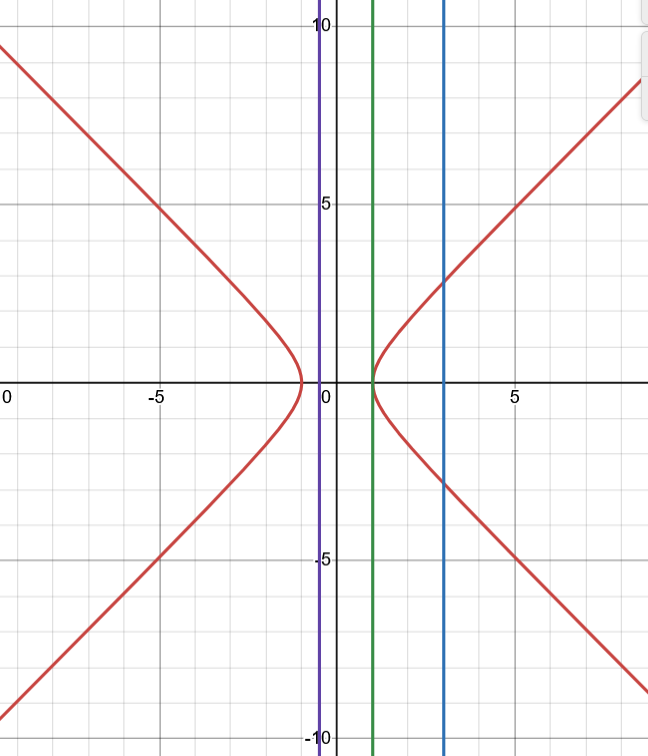
\includegraphics[width=0.5\linewidth]{cox-little-oshea/ch1/assets/sec1-3-ex5b.png}
            \caption{The hyperbola with the vertical lines $x=3$, $x=1$ and $x=1/2$.}
            \label{fig:sec1-3-ex5b}
        \end{figure}
        Next, we have the case of a nonvertical line $y=mx+b$. 
        We get:
        \begin{align*}
            1
            =& x^2 - y^2\\
            =& x^2 - (mx+b)^2\\
            =& x^2 - m^2 x^2 - 2mbx - b^2\\
            =& (1 - m^2)x^2 - 2mbx - b^2.
        \end{align*}
        We get the quadratic equation
        \begin{align*}
            (1-m^2)x^2 - 2mbx -(b^2 + 1) = 0.
        \end{align*}
        We have the discriminant
        \begin{align*}
            D = 4m^2 b^2 + 4(1-m^2)(b^2 + 1).
        \end{align*}
        According to whether this is positive, negative, or zero, we see that the lines have zero, one or two solutions. 
        This is illustrated in the following picture
\begin{figure}
    \centering
    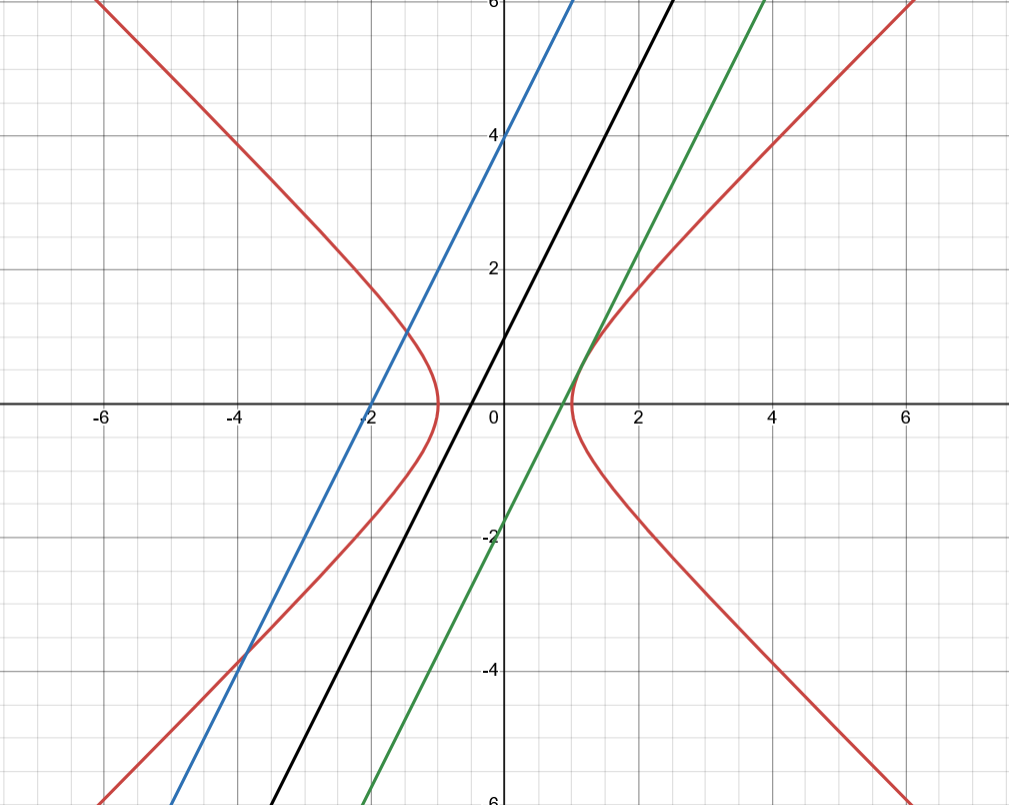
\includegraphics[width=0.5\linewidth]{cox-little-oshea/ch1/assets/sec1-3-ex5bb.png}
            \caption{The hyperbola with the lines $y = 2x+1$, $y=2x+4$ and $y = 2x-\sqrt{3}$.}
            \label{fig:sec1-3-ex5bb}
\end{figure}
        \item Let us consider a nonvertical line through the point $(-1,0)$ on the hyperbola. 
        Such a line as the form $y = mx + m$. 
        Let us plug this into the equation of the hyperbola:
        \begin{align*}
            1
            =& x^2 - y^2\\
            =& x^2 - (mx+m)^2\\
            =& x^2 - m^2 x^2 - 2m^2 x - m^2\\
            =& (1 - m^2) x^2 - 2m^2 x - m^2.
        \end{align*}
        Thus, we get the quadratic equation
        \begin{align*}
            0 
            = (1 - m^2) x^2 - 2m^2 x - (m^2 + 1) 
            = (x+1)( (1 - m^2)x-(1+m^2) ).
        \end{align*}
        The two intersection points are thus for $x=-1$ and
        \begin{align*}
            x = \frac{1 + m^2}{1 - m^2}.
        \end{align*}
        We get then that
        \begin{align*}
            y 
            = mx+m 
            = m\frac{1+m^2 + 1-m^2}{1-m^2} 
            = \frac{2m}{1-m^2}.
        \end{align*}
        We get the following parametrization:
        \begin{align*}
            x = \frac{1 + t^2}{1-t^2},~~y = \frac{2t}{1-t^2}.
        \end{align*}
        \item The parametrization is undefined for $1-t^2 = 0$, and thus $t=\pm 1$. 
        This corresponds to the lines $y=x+1$ and $y=-x-1$. 
        These lines are parallel to the asymptotes of the hyperbola. 
        The line will as such not intersect the hyperbola at any other point than $(-1,0)$.
    \end{enumerate}
\end{proof}

\begin{exercise}{6}
The goal of this problem is to show that the sphere $x^2+y^2+z^2=1$ in 3-dimensional space can be parametrised by
\begin{align*}
    x = \frac{2u}{u^2+v^2+1},\,\, 
    y = \frac{2v}{u^2+v^2+1},\,\, 
    z = \frac{u^2+v^2-1}{u^2+v^2+1}.
\end{align*}
The idea is to adapt the argument used for the circle $x^2+y^2=1$ to 3-dimensional space.
\begin{enumerate}
    \item Given a point $(u,v,0)$ in the $(x,y)$-plane, draw the line form this point to the ``north pole'' $(0,0,1)$ of the sphere, and let $(x,y,z)$ be the other point where the line meets the sphere. 
    Draw a picture to illustrate this, and argue geometrically that mapping $(u,v)$ to $(x,y,z)$ gives a parametrisation of the sphere minus the north pole.
    \item Show that the line connecting $(0,0,1)$ to $(u,v,0)$ is parametrised by $(tu,tv,1-t)$, where $t$ is a parameter that moves along the line.
    \item Substitute $x=tu, y=tv$ and $z=1-t$ into the equation for the sphere $x^2+y^2+z^2=1$. Use this to derive the formulas given at the beginning of the problem.
\end{enumerate}
\end{exercise}
\begin{proof}
\begin{enumerate}
    \item Since the described line intersects the unit sphere in only one point, and for all points of the sphere (besides $(0,0,1)$ we can find $u$ and $v$ so that the point of the sphere is the intersection with the line, then the whole sphere (with the exception of the north pole) is identified with $(u,v)$. 
    \begin{figure}[H]
     \centering
     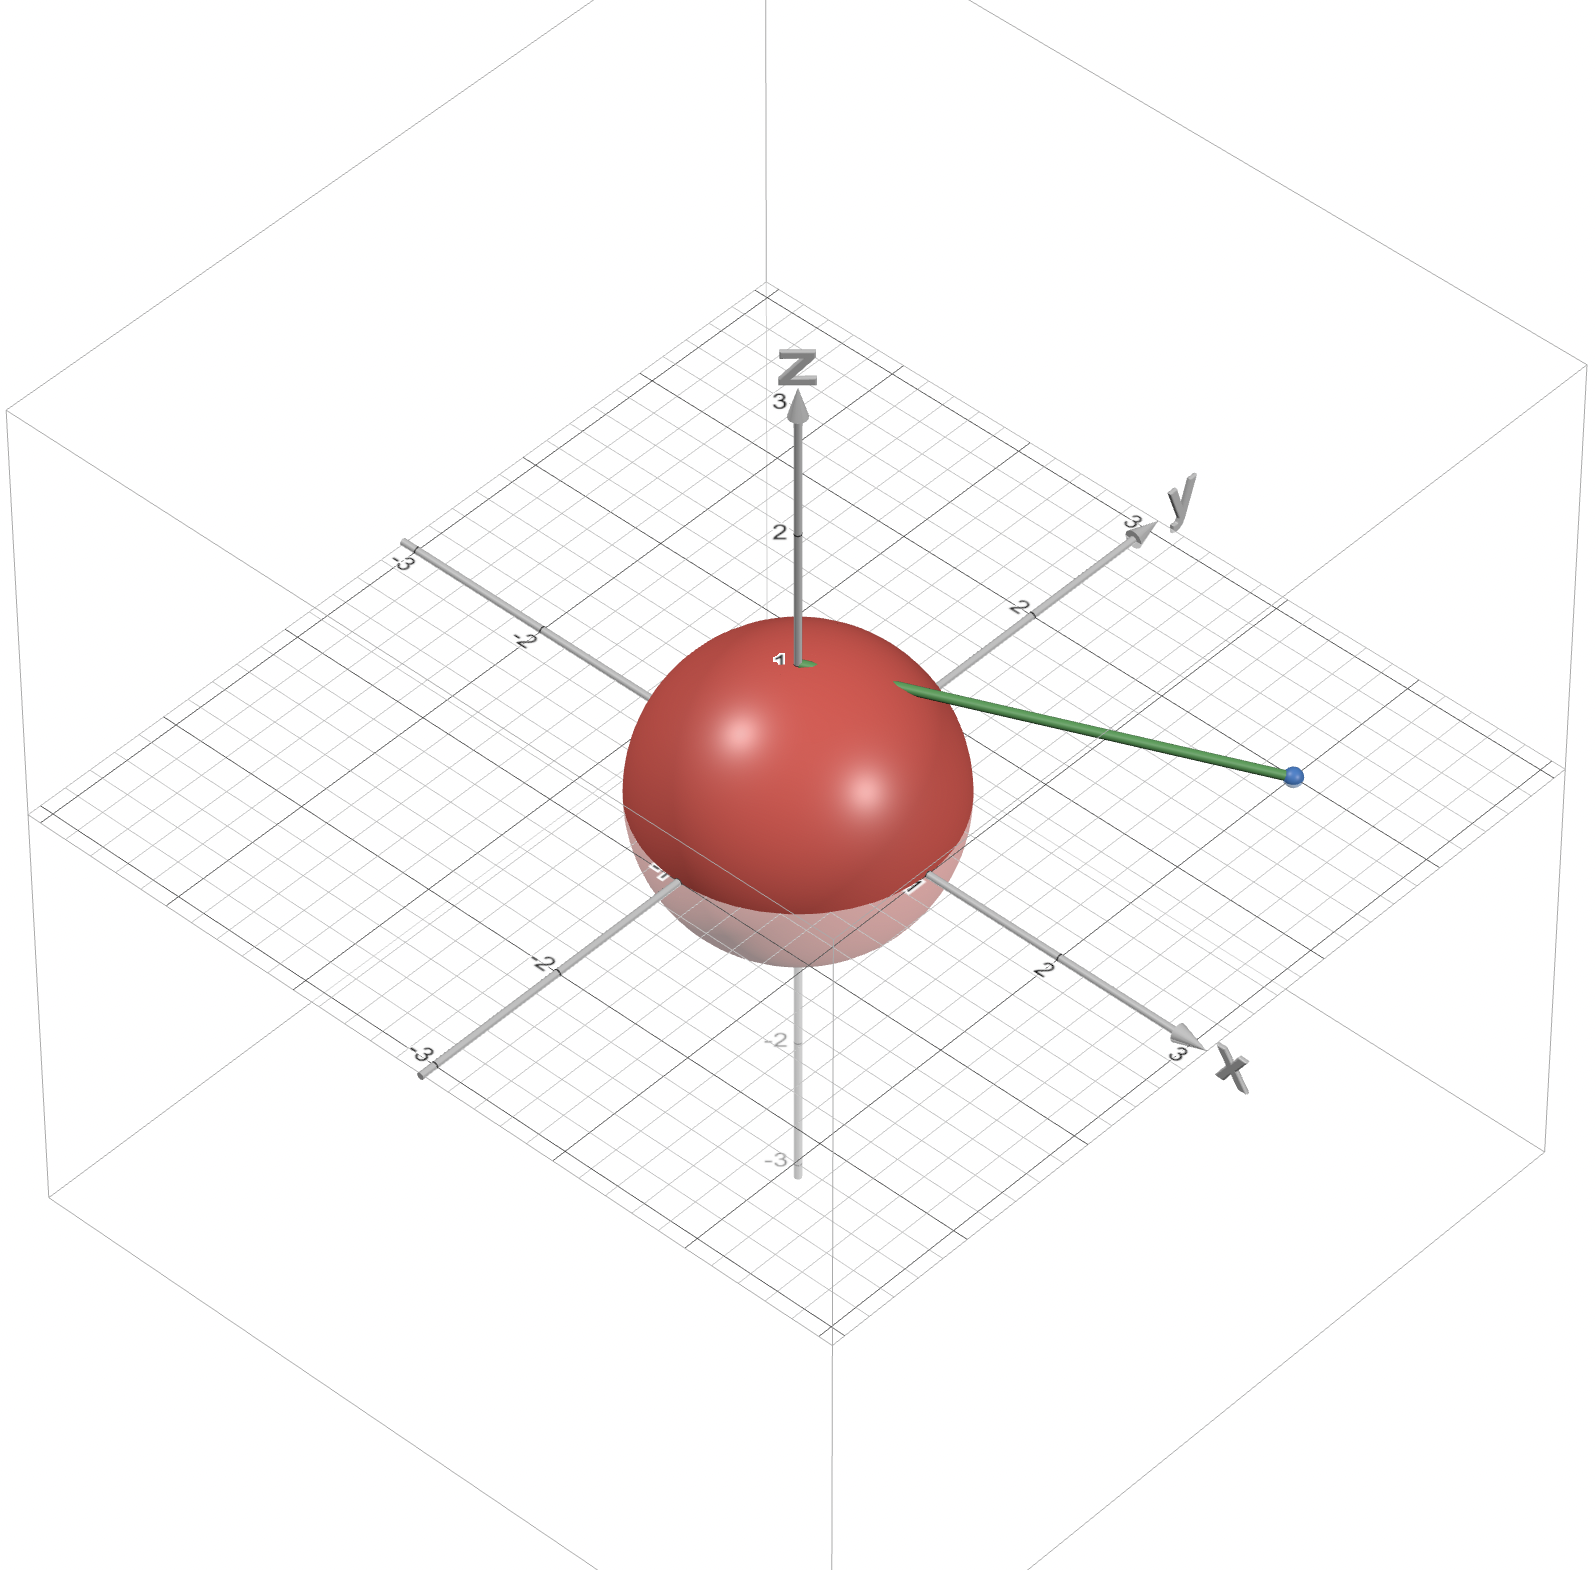
\includegraphics[width=.5\textwidth]{cox-little-oshea/ch1/assets/sec1-3-ex6a.png}
     \caption{Line between $(u,v,0)$ and $(0,0,1)$ for $u=v=2$ and the unit sphere.}
     \label{fig:sec1-3-ex8a}
    \end{figure}
    Remark: This appears on Brannan, Espen and Gray as the Stereographic projection.
    \item We know that the equation of a parametrised line in 3D is given by $r(t)=(x_0,y_0,z_0)+t(a,b,c)$, where $(a,b,c)$ are the slopes of the line. 
    We can find the slopes, given two points, by simply subtracting one point from the other. 
    We then have, $a=u, b=v$ and $c=-1$ then $r(t)=(0,0,1)+t(u,v,-1)=(tu,tv,1-t)$, as desired.
    \item We have 
    \begin{align*}
        &u^2t^2 + v^2t^2 + (1-t)^2 = 1 &&\iff\\
        &u^2t^2 + v^2t^2 + 1 - 2t + t^2 = 1 &&\iff\\
        &t^2(u^2 + v^2 + 1) - 2t = 0 &&\iff\\
        &t(u^2 + v^2 + 1) - 2 = 0 &&\iff\\
        &t = \frac{2}{u^2 + v^2 + 1}.
    \end{align*}
    Replacing $t$ in the above parametric equations of the line we obtain the desired result.
\end{enumerate}
\end{proof}

\begin{exercise}{7}
    Adapt the argument of the previous exercise to parametrize the ``sphere'' $x_1^2 + \dots + x_n^2 = 1$ in $n$-dimensional affine space.
\end{exercise}
\begin{proof}
    Given a point $(u_1,\dots,u_{n-1},0)$. 
    We draw the line to the ``north pole'' $(0,0,\dots,0,1)$ of the sphere and let $(x_1,\dots,x_n)$ be the other point where the line hits the sphere. The parametrization of said line is
    \begin{align*}
        x_1 = tu_1, \dots, x_{n-1} = tu_{n-1}, x_n = 1 - t.
    \end{align*}
    We want to find $t$. Plugging this in, we get
    \begin{align*}
        1
        =& x_1^2 + \dots + x_n^2\\
        =& (tu_1)^2 + \dots + (tu_{n-1})^2 + (1-t)^2\\
        =& t^2 (u_1^2 + \dots + u_{n-1})^2 + 1 - 2t + t^2.
    \end{align*}
    We get
    \begin{align*}
        t^2 (u_1^2 + \dots + u_{n-1}^2 + 1) - 2t = 0.
    \end{align*}
    Thus, we see that $t=0$ (which is the north pole), or
    \begin{align*}
        t = \frac{2}{u_1^2 + \dots + u_{n-1}^2 + 1}.
    \end{align*}
    We get
    \begin{align*}
        (x_1,\dots,x_n) 
        = \frac{(2u_1, \dots, 2 u_{n-1}, u_1^2 + \dots + u_{n-1}^2 -1)}{u_1^2 + \dots + u_{n-1}^2 + 1}.
    \end{align*}
    This is a parametrization of the $n-1$-sphere.
\end{proof}

\begin{exercise}{8}
Consider the curve defined by $y^2=cx^2-x^3$, where $c$ is some constant. Here is a picture of the curve when $c>0$:
\begin{figure}[H]
     \centering
     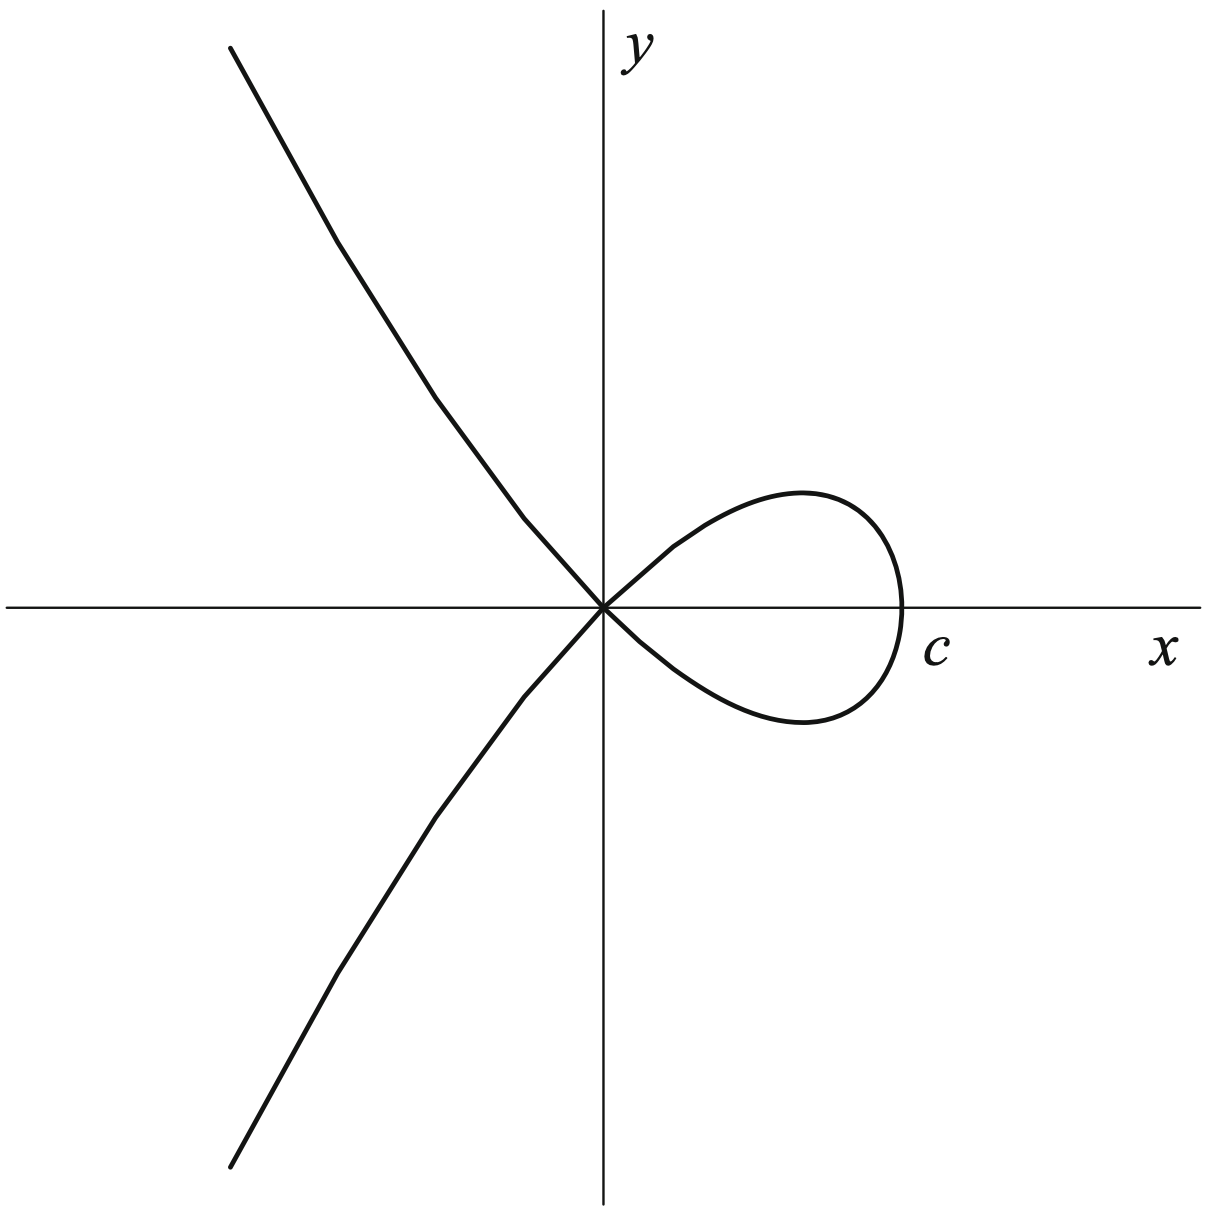
\includegraphics[width=.5\textwidth]{cox-little-oshea/ch1/assets/sec1-3-ex8.png}
     \label{fig:sec1-2-ex8}
\end{figure}
Our goal is to parametrise this curve.
\begin{enumerate}
    \item Show that a line will meet this curve at either 0, 1, 2, or 3 points. Illustrate your answer with a picture. 
    Hint: let the equation of the line be either $x=a$ or $y=mx+b$.
    \item Show that a nonvertical line through the origin meets the curve at exactly one other point when $m^2\neq c$. 
    Draw a picture to illustrate this, and see if you can come up with an intuitive explanation as to why this happens.
    \item Now draw the vertical line $x=1$. 
    Given a point $(1,t)$ on this line, draw the line connecting $(1,t)$ to the origin. 
    This will intersect the curve in a point $(x,y)$. Draw a picture to illustrate this, and argue geometrically that this gives a parametrisation of the entire curve.
    \item Show that the geometric description from part (3) leads to the parametrisation $x=c-t^2, y=t(c-t^2)$. 
\end{enumerate}
\end{exercise}
\begin{proof}
\begin{enumerate}
    \item Using the hint, consider the following two cases:

    Case 1. The line is vertical, with equation $x=a$. 
    Then we have
    \begin{align*}
        y^2 =& ca^2-a^3\\
        =& a^2(c-a)\implies\\
        y =& a\sqrt{c-a}.
    \end{align*}
    We then have two extra cases. 
    Case 1a: If $c-a\geq0$, then the line intersects the curve in the following two points $y=\pm a\sqrt{c-a}$, covering the 2 intersection case. 
    Case 1b: If $c-a<0$, then the line does not intersect the curve, covering the 0 case.

    Case 2. The line is given by the following function $y=mx+b$. 
    We have
    \begin{align*}
        &(mx+b)^2 = cx^2 -x^3 &&\implies\\
        &m^2x^2+2mbx+b^2 = cx^2-x^3 &&\implies\\
        &x^3+(m^2-c)x^2+2mbx+b^2 = 0 &&\text{(*)},
    \end{align*}
    which can have either 1 or 3 real roots (because complex roots come in pairs, covering the 1 or 3 intersection case.

    Cases 1a, 1b and 2 tell us that the lines can meet in 0, 1, 2 or 3 points.
    \item If $m^2\neq c$, and $b=0$ (because the line goes through the origin, we have that (*) is: $x^3+(m^2-c)x^2 = x^2(x+m^2-c)=0$, so that the roots of such polynomial are 0 and $x=c-m^2$. 
    
    My intuition of why this happens is that as we saw on (*), and replacing $b=0$, we must have 3 real roots, 0 being repeated. 
    Hence, we are only left with $x+m^2-c=0$ which is a single intersection between the curves.
    \begin{figure}[H]
         \centering
         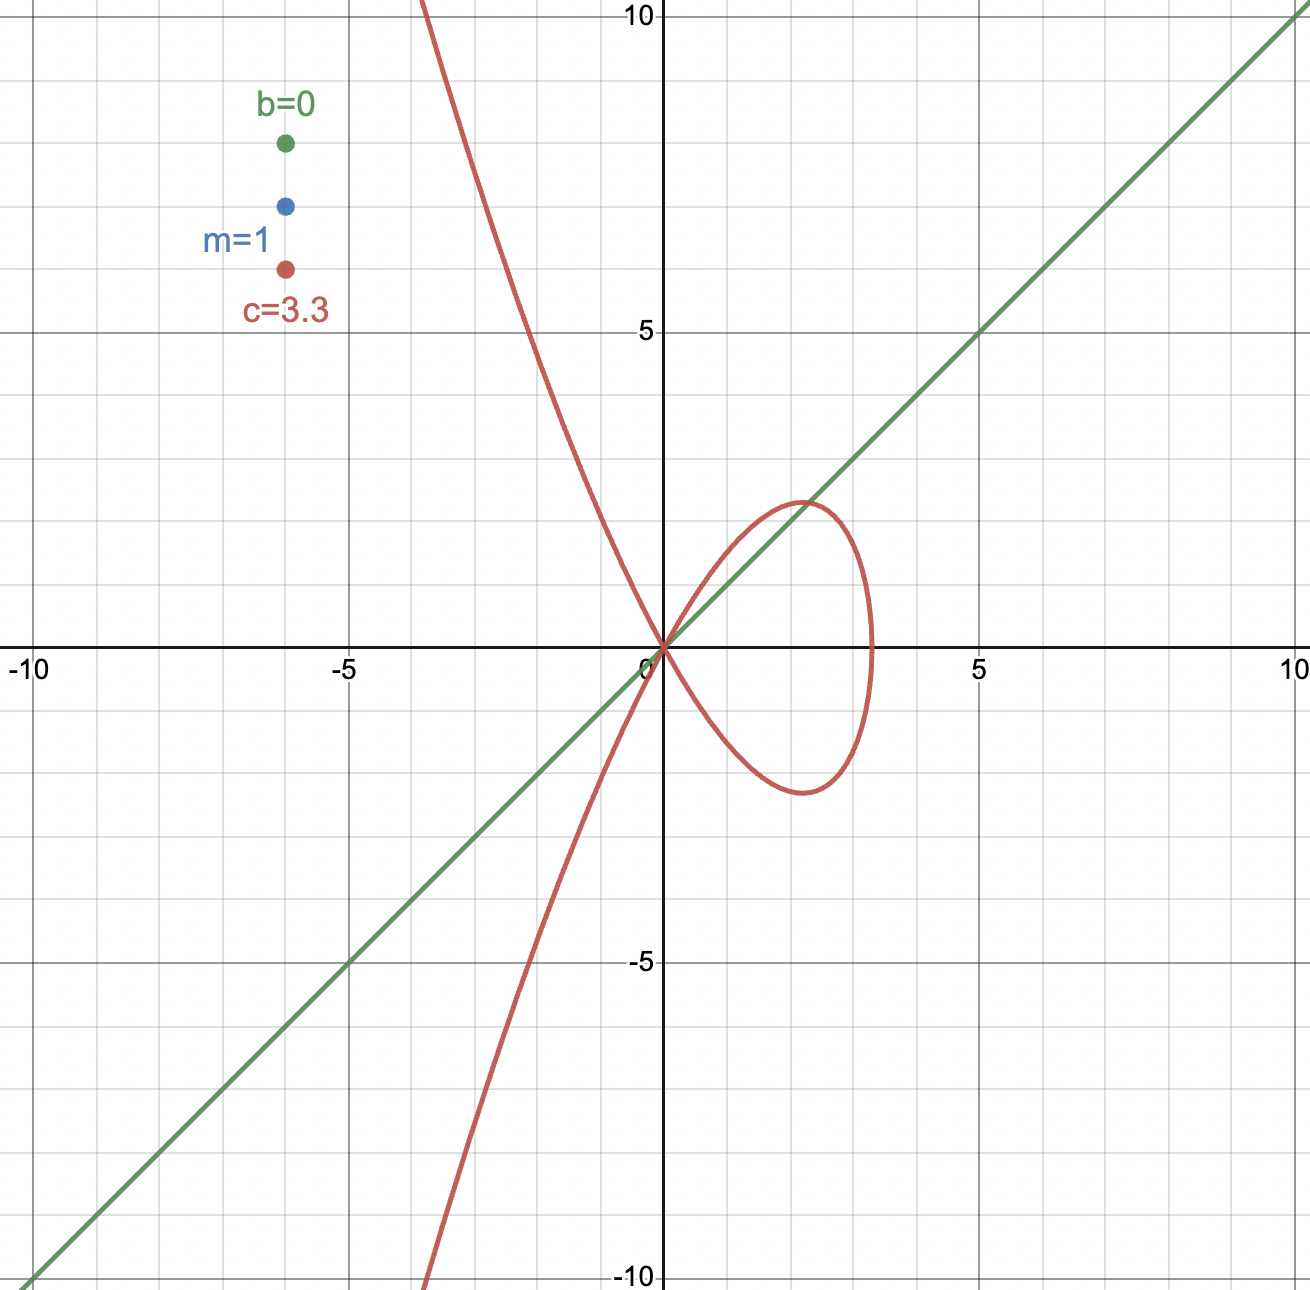
\includegraphics[width=.5\textwidth]{cox-little-oshea/ch1/assets/sec1-3-ex8-sol2.png}
         \label{fig:sec1-2-ex8-sol2}
    \end{figure}

    \item We just argued in the previous exercise that a line that goes through the origin meets the curve at a single point. 
    Geometrically, this is a parametrisation of the whole curve because the line through $(1,t)$ and the origin will have any slope we want, with functional form $y=mx$. 
    Since the intersection between this line and $y$ is given by (*) (with $b=0$), we cover all values of $y$. 
    To see this, just choose $(1,t)$ so that $m$ gives the desired value of $y$ whenever we replace $x=c-m^2$ in the original function of the equation.
    \begin{figure}[H]
         \centering
         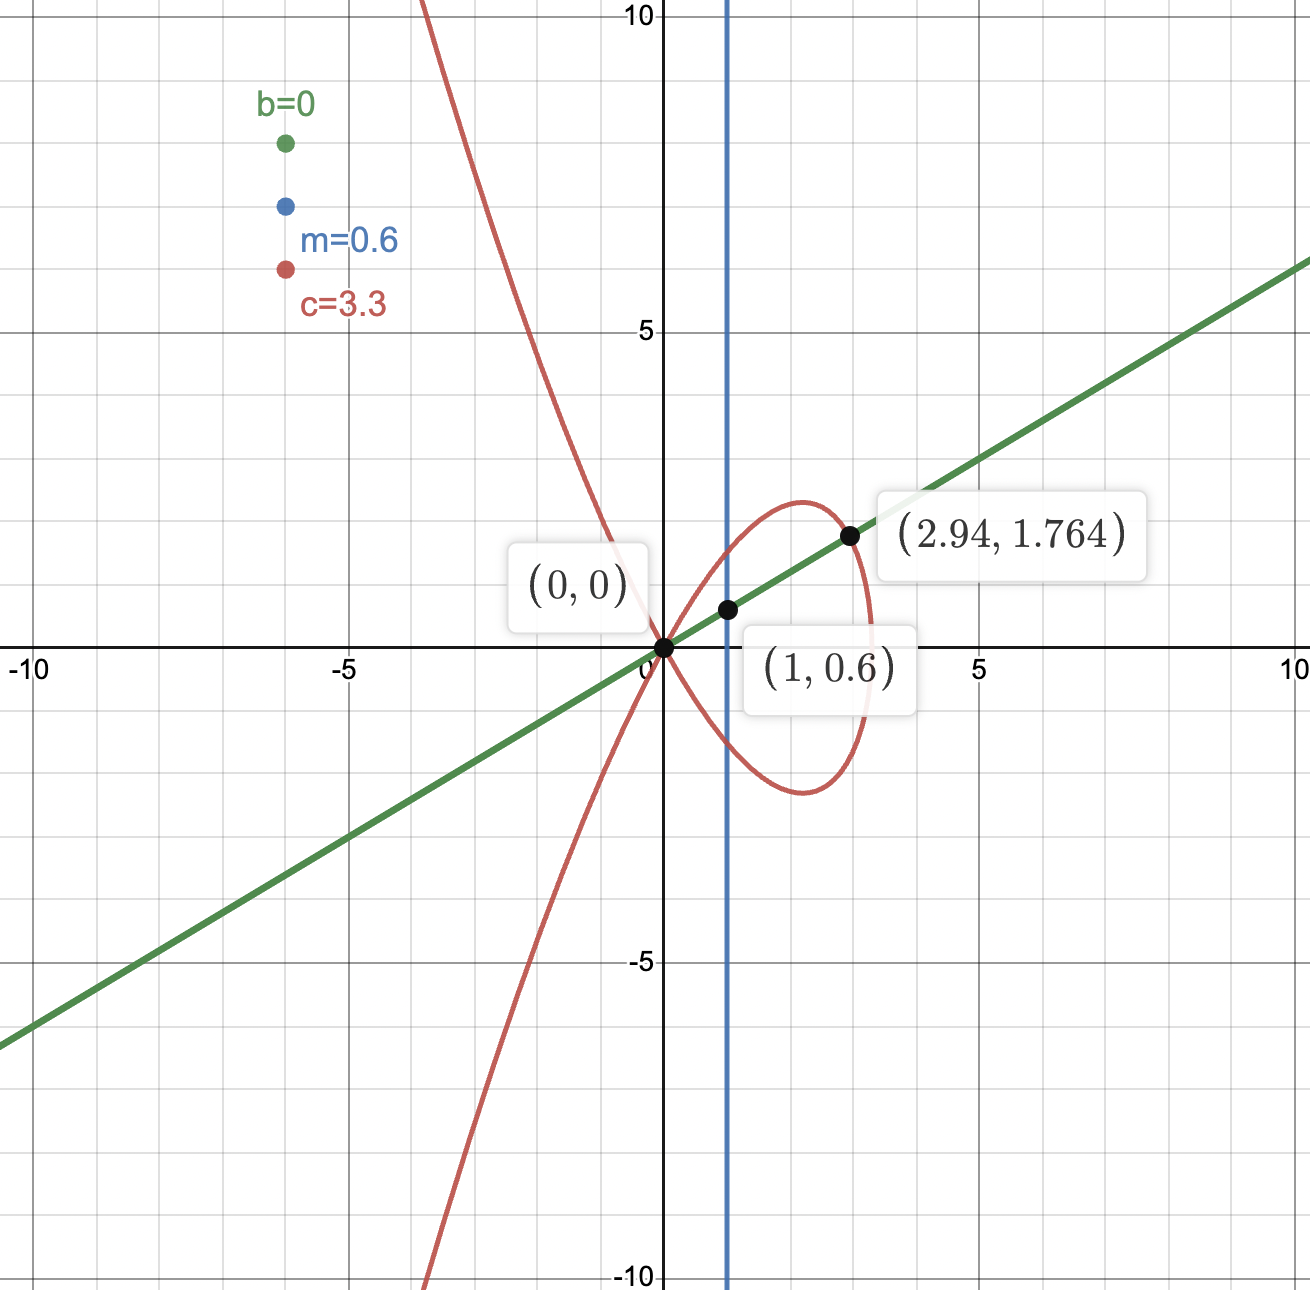
\includegraphics[width=.5\textwidth]{cox-little-oshea/ch1/assets/sec1-3-ex8-sol3.png}
         \label{fig:sec1-2-ex8-sol3}
    \end{figure}
    \item We just argued before about $x=c-m^2$, which translates to $x=c-t^2$ given that we are using the vertical curve $x=1$. 
    To see the parametrisation for $y$, we substitute as we intuitively argued above: 
    $y = \sqrt{c(c-t^2)^2-(c-t^2)^3} = \sqrt{t^2(c-t^2)^2} = t(c-t^2)$, as required.
\end{enumerate}
\end{proof}

\begin{exercise}{9}
The strophoid is a curve that was studied by various mathematicians, including Isaac Barrow ($1630-1677$), Jean Bernoulli ($1667-1748$), and Maria Agnesi ($1718-1799$). 
A trigonometric parametrization is given by
\begin{align*}
    x =& a\sin(t),\\
    y =& a\tan(t)( 1 + \sin(t) )
\end{align*}
where $a$ is a constant.
    \begin{enumerate}
        \item Find the equation in $x$ and $y$ that describes the strophoid.
        \item Find an algebraic parametrization of the strophoid.
    \end{enumerate}
\end{exercise}
\begin{proof}
    \begin{enumerate}
        \item We get that
        \begin{align*}
            y\cos t = a\sin t (1 + \sin t),
        \end{align*}
        and thus by squaring
        \begin{align*}
            y^2 \cos^2 t = a^2 \sin^2 t ( 1  + \sin t)^2,
        \end{align*}
        and thus
        \begin{align*}
            a^2 y^2 (1 - \sin^2 t) = a^2 \sin^2 t ( a + a\sin t)^2.
        \end{align*}
        Replacing $x=a\sin t$, we get
        \begin{align*}
            y^2 (a^2 - x^2) = x^2 (a + x)^2
        \end{align*}
        and thus
        \begin{align*}
            y^2 (a-x)(a+x) = x^2 (a+x)^2.
        \end{align*}
        Note however that $x+a = a(1 + \sin(t))$ only gives us zero when $t = -\pi/2 + 2k\pi$. 
        But in those points, $y$ is undefined. 
        So the curve never hits the line $x+a = 0$, which we can therefore cancel:
        \begin{align*}
            y^2 (a-x) = x^2 (a+x).
        \end{align*}
        Assume first that $a=0$, then we get $-y^2 x = x^3$. 
        If $x\neq 0$, then $-y^2 = x^2$, which cannot happen. 
        So only $(0,0)$ is in the graph, and clearly there is some $t$ such that $x=0\sin(t)$ and $y = a\tan(t) (1 + \sin(t))$.

        Next, assume that $a>0$. 
        Then if $x\geq a$, we see that $a-x\leq 0$ and $a+x>0$, which contradicts the equation $y^2 (a-x) = x^2 (a+x)$. 
        Similarly, if $x<-a$, then $a-x>0$ and $a+x<0$, contradicting the equation again. 
        Thus, we see that $-a\leq x<a$. We see that there is some $t\in (-3\pi/2,\pi/2)$ such that $a\sin(t) = x$. 
        Note that if $t=-\pi/2$, then $x=-a$ and thus $y=0$. 
        The equation $y = a\tan(t) (1+\sin(t))$ kind of makes sense in this case as well since you multiply by $0$. 
        In the case $t\neq -\pi/2$, we see that
        \begin{align*}
            y^2
            =& x^2\frac{a+x}{a-x}\\
            =& a^2 \sin^2 t \frac{a + a\sin t}{a - a\sin(t)}\\
            =& a^2 \sin^2 t \frac{1 + \sin(t)}{1 - \sin(t)}\\
            =& a^2 \sin^2 t \frac{(1 + \sin(t))^2}{1 - \sin^2(t)}\\
            =& a^2 \tan^2(t) (1 + \sin(t))^2.
        \end{align*}
        Thus, $y = a|\tan(t)|(1 + \sin(t))$. 
        Replacing $t$ by $\pi - t$ if necessary, we keep the equation $x = a\sin(t)$, but we can always assume $y = a\tan(t)(1+\sin(t))$ as well.

        The case $a<0$ is just the reflection of the case $-a>0$ over the $y$-axis and thus is handled similarly. 
        In each case, we see that the curve is described by the equation
        \begin{align*}
            y^2 (a-x) = x^2 (a+x).
        \end{align*}

        \item Let us consider the line $y=tx$ for a parameter $t$. We get
        \begin{align*}
            0 
            =& y^2 (a-x) - x^2 (a+x)\\
            =& t^2 x^2 (a-x) - x^2 (a+x)\\
            =& x^2 ( t^2(a-x) - (a+x))\\
            =& x^2 (  t^2 a - t^2 x - a - x)\\
            =& x^2 (  (t^2 - 1)a - (1+t^2) x).
        \end{align*}
        We see that $x=0$ or
        \begin{align*}
            x = \frac{t^2 - 1}{1 + t^2}.
        \end{align*}
        Then,
        \begin{align*}
            y = tx = \frac{t^3 - t}{1 + t^2}.
        \end{align*}
        It is clear by this construction that every point on the strophoid has a corresponding $t$.
    \end{enumerate}
\end{proof}

\begin{exercise}{10}
    Around $180$ B.C.E., Diocles wrote the book \emph{On Burning-Glasses}. 
    One of the curves he considered was the \emph{cissoid} and he used it to solve the problem of the duplication of the cube. 
    The cissoid has the equation $y^2 (a+x) = (a-x)^3$, where $a$ is a constant. 
    \begin{enumerate}
        \item Find an algebraic parametrization of the cissoid.
        \item Diocles described the cissoid using the following geometric construction. 
        Given a circle of radius $a$ (which we will take as centered at the origin), pick $x$ between $a$ and $-a$, and draw the line $L$ connecting $(a,0)$ to the point $P = (-x,\sqrt{a^2 - x^2})$ on the circle. 
        This determines a point $Q = (x,y)$ on $L$. 
        Prove that the cissoid is the locus of all such points $Q$.
        \item The duplication of the cube is the classical Greek problem of trying to construct $\sqrt[3]{2}$ using ruler and compass. 
        It is known that this is impossible given just a ruler and compass. 
        Diocles showed that if in addition, you allow the use of the cissoid, then one can construct $\sqrt[3]{2}$. 
        Here is how it works. 
        Draw the line connecting $(-a,0)$ to $(0,a/2)$. 
        This line will meet the cissoid at a point $(x,y)$. 
        Then prove that
        \begin{align*}
            2 = \left(\frac{a-x}{y}\right)^3,
        \end{align*}
         which shows how to construct $\sqrt[3]{2}$ using ruler, compass, and cissoid.
    \end{enumerate}
\end{exercise}
\begin{proof}
\begin{enumerate}
    \item A line through the point $(a,0)$ has the equation $y = t(x-a)$. 
    Thus, we get for the cissoid that
    \begin{align*}
        0
        =& y^2 (a+x) - (a-x)^3\\
        =& t^2 (a-x)^2 (a+x) - (a-x)^3\\
        =& (a-x)^2 ( t^2 (a+x) - (a-x))\\
        =& (a-x)^2 ( t^2 a + t^2 x - a + x)\\
        =& (a-x)^2 ( (1+t^2)x - (1 - t^2)a).
    \end{align*}
    Thus, we see that either $x=a$ or
    \begin{align*}
        x = \frac{1-t^2}{1+t^2}a,
    \end{align*}
    which also yields $x=a$ if $t=0$. 
    Then,
    \begin{align*}
        y = \frac{-2t^3}{1+t^2}a.
    \end{align*}
    \item The line through $(a,0)$ and $P$ has equation:
    \begin{align*}
        Y = \frac{\sqrt{a^2 - x^2}}{-x-a}(X-a).
    \end{align*}
    Plugging in $X = x$, we get
    \begin{align*}
        y^2
        =& \left(\frac{\sqrt{a^2 - x^2}}{-x-a}(x-a)\right)\\
        =& \frac{a^2 - x^2}{(x+a)^2}(x-a)^2\\
        =& \frac{(a-x)(a+x)}{(x+a)^2}(x-a)^2\\
        =& \frac{(a-x)}{x+a}(a-x)^2\\
        =& \frac{(a-x)^3}{x+a},
    \end{align*}
    giving the cissoid equation immediately.\\
    Conversely, assume that $y^2 (a+x) = (a-x)^3$. 
    Assume that $a>0$. 
    If $x>a$, then $a+x>0$ and $a-x\leq 0$, a contradiction. 
    Likewise, if $x\leq -a$, then $x+a\leq 0$ and $a-x>0$, a contradiction too. 
    We obtain that $x\in (-a,a]$. In particular, the following does not give a division by zero:
    \begin{align*}
        y^2
        =& \frac{(a-x)^3}{x+a}\\
        =& \frac{(a-x)}{x+a}(a-x)^2\\
        =& \frac{(a-x)(a+x)}{(x+a)^2}(x-a)^2\\
        =& \frac{a^2 - x^2}{(x+a)^2}(x-a)^2.    
    \end{align*}
    Since $a\in (-a,a]$, we know that $(x+a)/(x-a)\geq 0$, thus,
    \begin{align*}
        y = \frac{\sqrt{a^2 - x^2}}{-x-a}(x-a).
    \end{align*}
    Thus this is the point on the line
    \begin{align*}
        Y = \frac{\sqrt{a^2 - x^2}}{-x-a}(X-a)
    \end{align*}
    with $x$-coordinate $x$. 
    We get that thus that the point $(x,y)$ is obtained by the construction of Diocles.
    \item The line connecting $(-a,0)$ and $(0,a/2)$ is given by
    \begin{align*}
        y = \frac{a/2}{a}(x+a) = \frac{1}{2}(x+a).
    \end{align*}
    Plugging $x+a = 2y$ into the equation of the cissoid, we get
    \begin{align*}
        0
        =& y^2 (a+x) - (a-x)^3\\
        =& 2y^3 - (a-x)^3,
    \end{align*}
    from which we clearly get that
    \begin{align*}
        2 = \frac{(a-x)^3}{y^3}.
    \end{align*}
\end{enumerate}
\end{proof}

\begin{exercise}{11}
In this problem, we will derive the parametrisation
\begin{align*}
    x = t(u^2-t^2),\,\, y = u,\,\, z = u^2-t^2
\end{align*}
of the surface $x^2-y^2z^2+z^3=0$ considered in the text.
\begin{enumerate}
    \item Adapt the formulas in part (4) of exercise 8 to show that the curve $x^2 = cz^2-z^3$ is parametrized by 
    \begin{align*}
        z=c-t^2,\,\, x=t(c-t^2).
    \end{align*}
    \item Now replace the c in part (1) by $y^2$, and explain how this leads to the above parametrisation of $x^2-y^2z^2+z^3=0$.
    \item Explain why this parametrisation covers the entire surface $\bV(x^2-y^2z^2+z^3$. Hint: See part (3) of exercise 8.
\end{enumerate}
\end{exercise}
\begin{proof}
\begin{enumerate}
    \item These are exactly the same formulas as in part (4) of 8, where $x=y$ and $z=x$. 
    \item After replacing $c=y^2$, we have $x^2=y^2z^2-z^3$, which is exactly the parametrisation we want.
    \item As argued on the two previous solutions, the formulas here presented are the same as in Exercise 8 where $x=y$ and $z=x$. 
    Furthermore, instead of having $c$ as a parameter as in Exercise 8, we introduce a new variable to take on that value, namely $y^2=c$. 
    Since the reasons of why the parametrisation in Exercise 8 did not depend on the value of $c$, then we simply introduce a new variable, $y$, and parameter, $u$, without affecting the fact that the entire surface is covered by the parametrisation.
\end{enumerate}
\end{proof}

\begin{exercise}{12}
Consider the variety $V = \bV(y-x^2,z-x^4)\subseteq\mathbb{R}^3$.
\begin{enumerate}
    \item Draw a picture of $V$.
    \item Parametrize $V$ in a way similar to what we did with the twisted cubic.
    \item Parametrize the tangent surface of $V$.
\end{enumerate}
\end{exercise}
\begin{proof}
    \begin{enumerate}
        \item We get
        \begin{figure}[H]
            \centering
            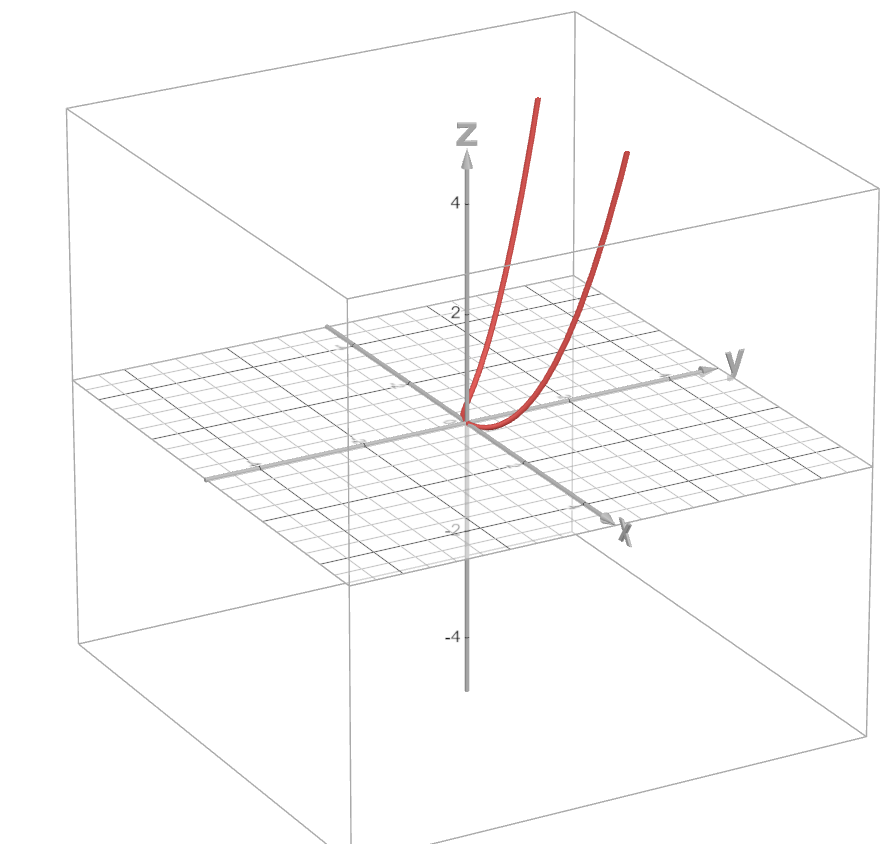
\includegraphics[width=0.5\linewidth]{cox-little-oshea/ch1/assets/sec1-3-ex12.png}
            \caption{Graph of the variety $V = \bV(y-x^2,z-x^4)$}
            \label{fig:sec1-3-ex12}
        \end{figure}
        \item It is clear the parametrization becomes
        \begin{align*}
            x =& t,\\
            y =& t^2,\\
            z =& t^4.
        \end{align*}
        Thus, $\mathbf{r}(t)= (t, t^2, t^4)$.
        \item Notice that the tangent vector at the point given by $\mathbf{r}(t)$ is 
        \begin{align*}
            \mathbf{r}'(t) = (1, 2t, 4t^3).
        \end{align*}
        It follows that the tangent line is parametrized by
        \begin{align*}
            \mathbf{r}(t) + u\mathbf{r}'(t) = (t + u, t^2 + 2tu, t^4 + 4t^3 u).
        \end{align*}
        Thus, we get the parametrization
        \begin{align*}
            x =& t+u\\
            y =& t^2 + 2tu\\
            z =& t^4 + 4t^3 u.
        \end{align*}
    \end{enumerate}
\end{proof}

\begin{exercise}{13}
The general problem of finding the equation of a parametrized surface will be studied in Chapters $2$ and $3$. 
However, when the surface is a plane, methods from calculus or linear algebra can be used. 
For example, consider the plane in $\mathbb{R}^3$ parametrized by
\begin{align*}
    x =& 1 + u - v,\\
    y =& u + 2v,\\
    z =& -1 - u + v.
\end{align*}
Find the equation of the plane determined this way.
\end{exercise}
\begin{proof}
    Let the equation of the plane by $ax+by+cz = d$. Hence,
    \begin{align*}
        d
        =& ax+by+cz\\
        =& a(1+u-v) + b(u + 2v) + c(-1 - u + v)\\
        =& (a-c) + u(a + b - c) + v(-a + 2b + c).
    \end{align*}
    We get a polynomial in $u$ and $v$ which has to be zero everywhere:
    \begin{align*}
        u(a + b - c) + v(-a + 2b + c) + (a-c-d) = 0.
    \end{align*}
    We then know that the coefficients must be zero, yielding the equations
    \begin{align*}
        a + b - c =& 0\\
        -a + 2b + c =& 0\\
        a -c - d = 0.
    \end{align*}
    Adding the first two equations gives us $b=0$. 
    We then get the following equations
    \begin{align*}
        a - c =& 0\\
        a - c - d =& 0,
    \end{align*}
    Giving us $a=c$ and $d = a - c = 0$. 
    We get that
    \begin{align*}
        x + z = 0
    \end{align*}
    is the equation of the plane.
\end{proof}

\begin{exercise}{14}
This problem deals with convex sets and will be used in the next exercise to show that a B\'ezier cubic lies within its control polygon. 
A subset $C\subseteq \mathbb{R}^2$ is convex if for all $P,Q\in C$, the line segment joining $P$ to $Q$ also lies in $C$.
\begin{enumerate}
    \item If 
    $P = 
    \left(\begin{array}{c} 
        x\\ 
        y
    \end{array}\right)$ 
    and 
    $Q = 
    \left(\begin{array}{c} 
        z\\ 
        w
    \end{array}\right)$ lie in a convex set $C$, then show that
    \begin{align*}
        t\left(\begin{array}{c} 
            x\\ 
            y\end{array}\right) 
        + (1-t)
        \left(\begin{array}{c} 
            z\\ 
            w\end{array}\right)
        \in C
    \end{align*}
    when $0\leq t\leq 1$.
    \item If 
    $P_i = 
    \left(\begin{array}{c} 
        x_i\\ 
        y_i\end{array}\right)$ 
    lies in a convex set $C$ for $1\leq i \leq n$, then show that
    \begin{align*}
        \sum_{i=1}^n t_i 
        \left(\begin{array}{c} 
            x_i\\ 
            y_i\end{array}\right)
        \in C
    \end{align*}
    wherever $t_1,\dots,t_n$ are nonnegative numbers such that $\sum_{i=1}^n t_i = 1$. 
\end{enumerate}
\end{exercise}
\begin{proof}
    \begin{enumerate}
        \item This is easy since the formula given is exactly a parametrization of the line segment through $P$ and $Q$.
        \item The statement is trivial for $n=1$. 
        Assume the statement is true for $n$, then take nonnegative numbers $t_1,\dots,t_{n+1}$ with $\sum_{i=1}^{n+1} t_i = 1$. 
        Then let 
        \begin{align*}
            s_i = \frac{t_i}{\sum_{k=1}^n t_k}.
        \end{align*}
        We see that $\sum_{i=1}^n s_i = 1$, and thus
        \begin{align*}
            \sum_{i=1}^n s_i \left(\begin{array}{c} x_i\\ y_i\end{array}\right)\in C.
        \end{align*}
        By part (a),
        \begin{align*}
            (1 - t_{n+1})\sum_{i=1}^n s_i 
            \left(\begin{array}{c} 
                x_i\\ 
                y_i\end{array}\right) 
            + t_{n+1}
            \left(\begin{array}{c} 
                x_{n+1}\\ 
                y_{n+1}\end{array}\right)
            \in C.
        \end{align*}
    
        But,
        \begin{align*}
            (1 - t_{n+1})\sum_{i=1}^n s_i 
            \left(\begin{array}{c} 
                x_i\\ 
                y_i\end{array}\right) 
            + t_{n+1}
            \left(\begin{array}{c} 
                x_{n+1}\\ 
                y_{n+1}\end{array}\right)
            =& \left(\sum_{i=1}^{n+1} t_i - t_{n+1}\right)\sum_{i=1}^n s_i 
            \left(\begin{array}{c} 
                x_i\\ 
                y_i\end{array}\right) 
            + t_{n+1}
            \left(\begin{array}{c} 
                x_{n+1}\\ 
                y_{n+1}\end{array}\right)\\
            =& \left(\sum_{i=1}^n t_i\right)\sum_{i=1}^n s_i 
            \left(\begin{array}{c} 
                x_i\\ 
                y_i\end{array}\right) 
            + t_{n+1}
            \left(\begin{array}{c} 
                x_{n+1}\\ 
                y_{n+1}\end{array}\right)\\
            =& \left(\sum_{i=1}^n t_i\right)\sum_{i=1}^n \frac{t_i}{\sum_{k=1}^n t_k} \left(\begin{array}{c} 
                x_i\\ 
                y_i\end{array}\right) 
            + t_{n+1}
            \left(\begin{array}{c} 
                x_{n+1}\\ 
                y_{n+1}\end{array}\right)\\
            =& \sum_{i=1}^n t_i 
            \left(\begin{array}{c} 
                x_i\\ 
                y_i\end{array}\right) 
            + t_{n+1}
            \left(\begin{array}{c} 
                x_{n+1}\\ 
                y_{n+1}\end{array}\right)\\
            =& \sum_{i=1}^{n+1} t_i 
            \left(\begin{array}{c} 
                x_i\\ 
                y_i\end{array}\right).
        \end{align*}
        This proves the induction.
    \end{enumerate}
\end{proof}

\begin{exercise}{15}
    Let a B\'ezier cubic be given by
    \begin{align*}
        x =& (1-t)^3 x_0 + 3t(1-t)^2 x_1 + 3t^2 (1-t) x_2 + t^3 x_3,\\
        x =& (1-t)^3 y_0 + 3t(1-t)^2 y_1 + 3t^2 (1-t) y_2 + t^3 y_3.        
    \end{align*}
    
    \begin{enumerate}
        \item Show that the above equations can be written in vector form
        \begin{align*}
            \parens{
            \begin{array}{c} 
                x\\ 
                y
            \end{array}}
            = (1-t)^3 
            \parens{
            \begin{array}{c} 
                x_0\\ 
                y_0
            \end{array}} 
            + 3t(1-t)^2 
            \parens{
            \begin{array}{c} 
                x_1\\ 
                y_1
            \end{array}} 
            + 3t^2 (1-t) 
            \parens{
            \begin{array}{c} 
                x_2\\ 
                y_2
            \end{array}} 
            + t^3 
            \parens{
            \begin{array}{c} 
                x_3\\ 
                y_3
            \end{array}}.
        \end{align*}
        \item Use the previous exercise to show that a B\'{e}zier cubic always lies inside its control polygon.
    \end{enumerate}
\end{exercise}
\begin{proof}
    \begin{enumerate}
        \item This is trivial by looking at the equation in the two components. 
        \item We see that
        \begin{align*}
            (1-t)^3 + 3t(1-t)^2 + 3t^2 (1-t) + t^3
            =& ( (1-t) + t)^3\\
            =& 1^3\\
            =& 1.
        \end{align*}
        Thus, since the sum of the coefficients is $1$, and the control polygon is by definition convex, we see that $(x,y)$ lies in the control polygon for all $t$.
    \end{enumerate}
\end{proof}

\begin{exercise}{16}
One disadvantage of B\'ezier cubics is that curves like circles and hyperbolas cannot be described exactly by cubics. 
In this exercise, we will discuss a method similar to example (4) for parametrizing conic sections.

A conic section is a curve in the plane defined by a second degree equation of the form $ax^2 + bxy + cy^2 + dx + ey = 0$. 
Conic sections include the familiar examples of circles, ellipses, parabolas, and hyperbolas. 
Now consider the curve parametrized by
\begin{align*}
    x =& \frac{(1-t)^2 x_1 + 2t(1-t)wx_2 + t^2 x_3}{(1-t)^2 + 2t(1-t)w + t^2},\\
    y =& \frac{(1-t)^2 y_1 + 2t(1-t)wy_2 + t^2 y_3}{(1-t)^2 + 2t(1-t)w + t^2}    
\end{align*}
for $0\leq t\leq 1$. 
The constants $w,x_1,y_1,x_2,y_2,x_3,y_3$ are specified by the design engineer, and we will assume that $w\geq 0$. 
In Chapter $3$, we will show that these equations parametrize a conic section. 
The goal of this exercise is to give a geometric interpretation for the quantities $w,x_1,y_1,x_2,y_2,x_3,y_3$.
    \begin{enumerate}
        \item Show that our assumption $w\geq 0$ implies that the denominator in the above formulas never vanishes.
        \item Evaluate the above formulas at $t=0$ and $t=1$. 
        This should tell you what $x_1$, $y_1$, $x_3$, $y_3$ mean.
        \item Now compute $(x'(0), y'(0))$ and $(x'(1), y'(1))$. 
        Use this to show that $(x_2,y_2)$ is the intersection of the tangent lines at the start and end of the curve. 
        Explain why $(x_1,y_1)$, $(x_2,y_2)$ and $(x_3,y_3)$ are called the control points of the curve.
        \item Define the control polygon (it is actually a triangle in this case), and prove that the curve defined by the above equations always lies in its control polygon. 
        This gives the following picture:
        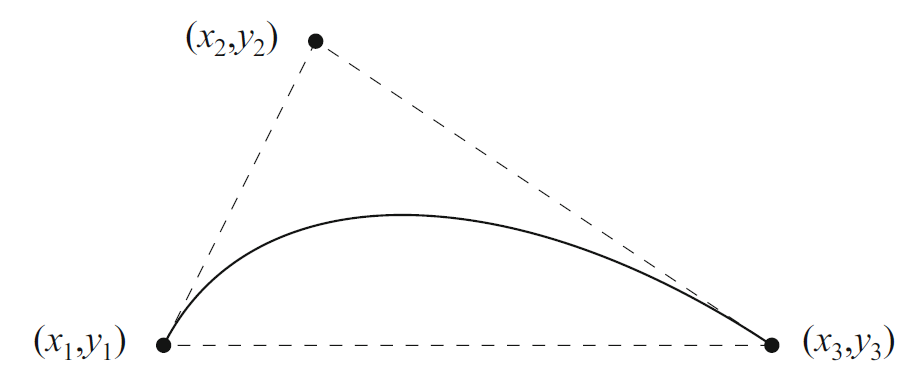
\includegraphics[width=0.8\linewidth]{cox-little-oshea/ch1/assets/sec1-3-ex16.png}
        It remains to explain the constant $w$, which is called the shape factor. 
        A hint should come from the answer to part (c), for note that $w$ appears in the formulas for the tangent vectors when $t=0$ and $1$. 
        So $w$ somehow controls the ``velocity,'' and a larger $w$ should force the curve closer to $(x_2,y_2)$. 
        In the last two parts of the problem, we will determine exactly what $w$ does.
        \item Prove that
        \begin{align*}
            \left(\begin{array}{c}
                x
                \left(\frac{1}{2}\right)\\ 
                y\left(\frac{1}{2}\right)
            \end{array}\right) 
            = \frac{1}{1+w}\left(\frac{1}{2}
                \left(\begin{array}{c}
                    x_1\\ 
                    y_1\end{array}\right) 
                + \frac{1}{2}
                \left(\begin{array}{c}
                    x_3\\ 
                    y_3\end{array}\right) \right) 
                + \frac{w}{1+w}
                \left(\begin{array}{c}
                    x_2\\ 
                    y_2\end{array}\right).
        \end{align*}
        Use this formula to show that $\left(x\left(\frac{1}{2}\right),y\left(\frac{1}{2}\right)\right)$ lies on the line segment connecting $(x_2,y_2)$ to the midpoint between $(x_1,y_1)$ and $(x_3,y_3)$.
        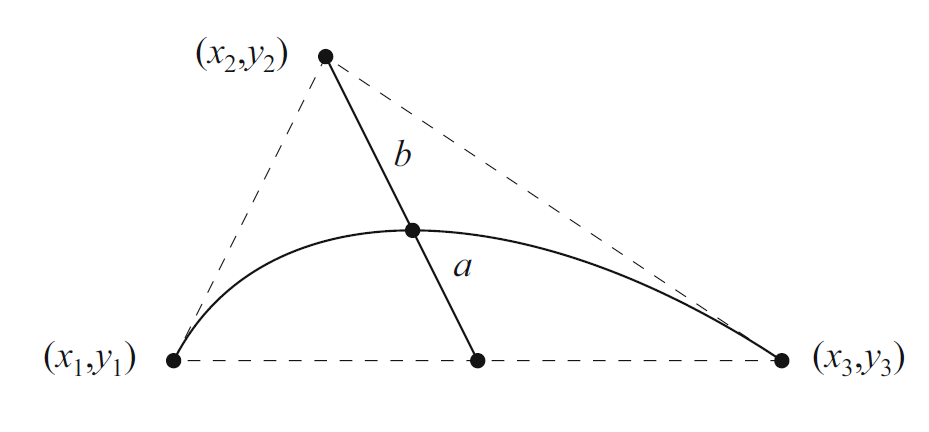
\includegraphics[width=0.8\linewidth]{cox-little-oshea/ch1/assets/sec1-3-ex16a.png}
        \item Notice that $\left(x\left(\frac{1}{2}\right), y\left(\frac{1}{2}\right)\right)$ divides this line segment into two pieces, say of length $a$ and $b$ as indicated in the above picture. Then prove that
        \begin{align*}
            w = \frac{a}{b},
        \end{align*}
        so that $w$ tells us exactly where the curve crosses this line segment.
    \end{enumerate}
\end{exercise}
\begin{proof}
    \begin{enumerate}
        \item Since $w\geq 0$, we see that
        \begin{align*}
            (1-t)^2 + 2t(1-t)w + t^2\geq (1-t)^2 + t^2 > 0.
        \end{align*}
        \item As $t=0$, we get
        \begin{align*}
            x & = \frac{(1-t)^2 x_1 + 2t(1-t)wx_2 + t^2 x_3}{(1-t)^2 + 2t(1-t)w + t^2} & = x_1,\\
            y & = \frac{(1-t)^2 y_1 + 2t(1-t)wy_2 + t^2 y_3}{(1-t)^2 + 2t(1-t)w + t^2} & = y_1.
        \end{align*}        
        We get for $t=1$, that
        \begin{align*}
            x & = \frac{(1-t)^2 x_1 + 2t(1-t)wx_2 + t^2 x_3}{(1-t)^2 + 2t(1-t)w + t^2} & = x_3,\\
            y & = \frac{(1-t)^2 y_1 + 2t(1-t)wy_2 + t^2 y_3}{(1-t)^2 + 2t(1-t)w + t^2} & = y_3. 
        \end{align*}     
        So we see that $(x_1,y_1)$ and $(x_3, y_3)$ are the begin and endpoints of the segment.
        \item We see that 
        \begin{align*}
            x'(t) 
            = \frac{2w(-x_1(t-1)^2 + 2x_2t + x_2 + x_3t^2) + 2(t-1)t(x_1 - x_3)}{(1 - 2(t-1)t(w-1))^2}.
        \end{align*}
        We get,
        \begin{align*}
            x'(0) 
            = 2w(x_2 - x_1),y'(0) 
            = 2w(x_3 - x_2).
        \end{align*}
        Similarly,
        \begin{align*}
            y'(0) 
            = 2w(y_2 - y_1),y'(0) 
            = 2w(y_3 - y_2).
        \end{align*}
        The tangent line through $(x_1, y_1)$, is given by
        \begin{align*}
            f(t) 
            = (x(0),y(0)) + t(x'(0),y'(0)) 
            = (x_1 + 2wt (x_2 - x_1), y_1 + 2wt(y_2 - y_1)).
        \end{align*}
        Putting $t= \frac{1}{2w}$, we get that $(x_2,y_2)$ is on this tangent line. 
        Similarly, it is on the tangent line $g(t) = (x(1),y(1)) + t(x'(1),y'(1))$. 
        This establishes that $(x_2,y_2)$ is on the intersection of the two tangent lines. 
        We say that $(x_1,y_1)$, $(x_2, y_2)$ and $(x_3,y_3)$ are called the control points since they control completely geometrically what the curve looks like.
        \item We can write
        \begin{align*}
            \left(\begin{array}{c} 
                x\\ 
                y \end{array}\right) 
            =& \frac{(1-t)^2}{(1-t)^2 + 2t(1-t)w + t^2}
            \left(\begin{array}{c} 
                x_1\\ 
                y_1 \end{array}\right)\\
            & +\frac{2t(1-t)w}{(1-t)^2 + 2t(1-t)w + t^2}
            \left(\begin{array}{c} 
                x_2\\ 
                y_2  \end{array}\right)\\
            & + \frac{t^2}{(1-t)^2 + 2t(1-t)w + t^2}
            \left(\begin{array}{c} 
                x_1\\ 
                y_1 \end{array}\right).
        \end{align*}
        Note that each of the three coefficients is in $[0,1]$, and they clearly add up to $1$. 
        Thus since $(x,y)$ is a convex combination of $(x_1,y_1)$, $(x_2,y_2)$ and $(x_3,y_3)$, we see that $(x,y)$ is in the control polygon.
        \item We see that
        \begin{align*}
           x\left(\frac{1}{2}\right)
           =& \frac{\left(1-\frac{1}{2}\right)^2 x_1 + 2\frac{1}{2}\left(1-\frac{1}{2}\right)wx_2 + \left(\frac{1}{2}\right)^2 x_3}{\left(1-\frac{1}{2}\right)^2 + 2\frac{1}{2}\left(1-\frac{1}{2}\right)w + \left(\frac{1}{2}\right)^2}\\
           =& \frac{\left(\frac{1}{2}\right)^2 x_1 + 2\frac{1}{2}\left(\frac{1}{2}\right)wx_2 + \left(\frac{1}{2}\right)^2 x_3}{\left(\frac{1}{2}\right)^2 + 2\frac{1}{2}\left(\frac{1}{2}\right)w + \left(\frac{1}{2}\right)^2}\\
           =& \frac{\frac{1}{4} x_1 + 2\frac{1}{4}wx_2 + \frac{1}{4} x_3}{\frac{1}{4} + 2\frac{1}{4}w + \frac{1}{4}}\\
           =& \frac{\frac{1}{4} x_1 + \frac{1}{2}wx_2 + \frac{1}{4} x_3}{\frac{1}{2} + \frac{1}{2}w}\\
           =& \frac{\frac{1}{2} x_1 + wx_2 + \frac{1}{2} x_3}{1+w}\\
           =& \frac{1}{2}\frac{x_1}{1+w} + \frac{w}{1+w}x_2 + \frac{1}{2}\frac{x_3}{1+w}\\
           =& \frac{1}{1+w}\left(\frac{1}{2}x_1 + \frac{1}{2}x_3\right) + \frac{w}{1+w}x_3.
        \end{align*}
        A similar computation holds for $y\left(\frac{1}{2}\right)$.
            \item The midpoint between $(x_1,y_1)$ and $(x_3,y_3)$ has coordinates 
            \begin{align*}
                \left(\begin{array}{c}
                    x_{\text{mid}}\\ 
                    y_{\text{mid}}\end{array}\right) 
                = \frac{1}{2}
                \left(\begin{array}{c}
                    x_1\\ 
                    y_1\end{array}\right) 
                + \frac{1}{2}
                \left(\begin{array}{c}
                    x_3\\ 
                    y_3\end{array}\right).
            \end{align*}
            Thus,
            \begin{align*}
                \left(\begin{array}{c}
                    x\left(\frac{1}{2}\right)\\ 
                    y\left(\frac{1}{2}\right)\end{array}\right) 
                = \frac{1}{1+w}
                \left(\begin{array}{c}
                    x_{\text{mid}}\\ 
                    y_{\text{mid}}\end{array}\right) 
                + \frac{w}{1+w}
                \left(\begin{array}{c}
                    x_2\\ 
                    y_2\end{array}\right).
            \end{align*}
            By Exercise $14$ and choosing $t = \frac{1}{1+w}$, we then see that $\left(x\left(\frac{1}{2}\right),y\left(\frac{1}{2}\right)\right)$ is part of the line going through $(x_{\text{mid}},y_{\text{mid}})$ and $(x_2,y_2)$, as desired.
            \item Note that
            \begin{align*}
                \frac{a}{b}
                =& \frac{\left\|\left(\begin{array}{c} x\left(\frac{1}{2}\right)\\ y\left(\frac{1}{2}\right)\end{array}\right) 
                - \left(\begin{array}{c} x_{\text{mid}}\\ y_{\text{mid}}\end{array}\right)\right\|}{\left\|\left(\begin{array}{c} x\left(\frac{1}{2}\right)\\ y\left(\frac{1}{2}\right)\end{array}\right) 
                - \left(\begin{array}{c} x_2\\ y_2\end{array}\right)\right\|}\\
                =& \frac{\left\|\frac{1}{1+w}\left(\begin{array}{c} x_{\text{mid}}\\ y_{\text{mid}}\end{array}\right) 
                + \frac{w}{1+w}\left(\begin{array}{c} x_2\\ y_2\end{array}\right) 
                - \left(\begin{array}{c} x_{\text{mid}}\\ y_{\text{mid}}\end{array}\right)\right\|}{\left\|\frac{1}{1+w}\left(\begin{array}{c} x_{\text{mid}}\\ y_{\text{mid}}\end{array}\right) + \frac{w}{1+w}\left(\begin{array}{c} x_2\\ y_2\end{array}\right) 
                - \left(\begin{array}{c} x_2\\ y_2\end{array}\right)\right\|}\\        
                =& \frac{\left\|-\frac{w}{1+w}\left(\begin{array}{c} x_{\text{mid}}\\ y_{\text{mid}}\end{array}\right) 
                + \frac{w}{1+w}\left(\begin{array}{c} x_2\\ y_2\end{array}\right)\right\|}{\left\|\frac{1}{1+w}\left(\begin{array}{c} x_{\text{mid}}\\ y_{\text{mid}}\end{array}\right) 
                - \frac{1}{1+w}\left(\begin{array}{c} x_2\\ y_2\end{array}\right)\right\|}\\
                =& \frac{\frac{w}{1+w}\left\|-\left(\begin{array}{c} x_{\text{mid}}\\ y_{\text{mid}}\end{array}\right) 
                + \left(\begin{array}{c} x_2\\ y_2\end{array}\right)\right\|}{\frac{1}{1+w}\left\|\left(\begin{array}{c} x_{\text{mid}}\\ y_{\text{mid}}\end{array}\right) 
                - \left(\begin{array}{c} x_2\\ y_2\end{array}\right)\right\|}\\        
                =& w\frac{\left\|\left(\begin{array}{c} x_{\text{mid}}\\ y_{\text{mid}}\end{array}\right) 
                - \left(\begin{array}{c} x_2\\ y_2\end{array}\right)\right\|}{\left\|\left(\begin{array}{c} x_{\text{mid}}\\ y_{\text{mid}}\end{array}\right) 
                - \left(\begin{array}{c} x_2\\ y_2\end{array}\right)\right\|}\\        
                =& w.
            \end{align*}
    \end{enumerate}
\end{proof}

\begin{exercise}{17}
    Use the formulas of the previous exercise to parametrize the arc of the circle $x^2 + y^2 = 1$ from $(1,0)$ to $(0,1)$.
\end{exercise}
\begin{proof}
We see that
\begin{align*}
    (x_1,y_1) = (1,0),~(x_2,y_2) = (1,1),~(x_3,y_3) = (0,1).
\end{align*}
Also,
\begin{align*}
    (x_{\text{mid}}, y_{\text{mid}}) 
    = \left(\frac{1}{2}, \frac{1}{2}\right),~~\left(x\left(\frac{1}{2}\right), y\left(\frac{1}{2}\right)\right) 
    = \left(\frac{1}{\sqrt{2}},\frac{1}{\sqrt{2}}\right).
\end{align*}
Note then that
\begin{align*}
    w
    =& \frac{a}{b}\\
    =& \frac{\left\|\left(\begin{array}{c} x\left(\frac{1}{2}\right)\\ y\left(\frac{1}{2}\right)\end{array}\right) 
    - \left(\begin{array}{c} x_{\text{mid}}\\ y_{\text{mid}}\end{array}\right)\right\|}{\left\|\left(\begin{array}{c} x\left(\frac{1}{2}\right)\\ y\left(\frac{1}{2}\right)\end{array}\right) 
    - \left(\begin{array}{c} x_2\\ y_2\end{array}\right)\right\|}\\
    =& \frac{\left\|\left(\begin{array}{c} \frac{1}{\sqrt{2}}\\ \frac{1}{\sqrt{2}}\end{array}\right) 
    - \left(\begin{array}{c} \frac{1}{2}\\ \frac{1}{2}\end{array}\right)\right\|}{\left\|\left(\begin{array}{c} \frac{1}{\sqrt{2}}\\ \frac{1}{\sqrt{2}}\end{array}\right) 
    - \left(\begin{array}{c} 1\\ 1\end{array}\right)\right\|}\\
    =& \frac{\left\|\left(\begin{array}{c} \frac{1}{\sqrt{2}} 
    - \frac{1}{2}\\ \frac{1}{\sqrt{2}} - \frac{1}{2}\end{array}\right)\right\|}{\left\|\left(\begin{array}{c} \frac{1}{\sqrt{2}} 
    - 1\\ \frac{1}{\sqrt{2}} 
    - 1\end{array}\right)\right\|}\\
    =& \frac{\sqrt{\left(\frac{1}{\sqrt{2}} 
    - \frac{1}{2}\right)^2 + \left(\frac{1}{\sqrt{2}} - \frac{1}{2}\right)^2}}{\sqrt{\left(\frac{1}{\sqrt{2}} - 1\right)^2 + \left(\frac{1}{\sqrt{2}} - 1\right)^2}}\\
    =& \frac{\frac{1}{\sqrt{2}} - \frac{1}{2}}{1 \frac{1}{\sqrt{2}}}\\
    =& \frac{\frac{2 - \sqrt{2}}{2\sqrt{2}}}{\frac{\sqrt{2} - 1}{\sqrt{2}}}\\
    =& \frac{2 - \sqrt{2}}{2\sqrt{2} - 2}\\
    =& \frac{(2 - \sqrt{2})(1 + \sqrt{2})}{2(2 - 1)}\\
    =& \frac{1}{2}(2 + 2\sqrt{2} - \sqrt{2} - 2)\\
    =& \frac{\sqrt{2}}{2}\\
    =& \frac{1}{\sqrt{2}}.    
\end{align*}
So,
\begin{align*}
    x 
    = \frac{(1- t)^2 x_1 + 2t(1-t)wx_2 + t^2 x_3}{(1- t)^2 + 2t(1-t)w + t^2} 
    = \frac{(1- t)^2 + \sqrt{2}t(1-t)}{(1- t)^2 + \sqrt{2}t(1-t) + t^2}
\end{align*}
and
\begin{align*}
    x = \frac{(1- t)^2 y_1 + 2t(1-t)wy_2 + t^2 y_3}{(1- t)^2 + 2t(1-t)w + t^2} = \frac{\sqrt{2}t(1-t) + t^2}{(1- t)^2 + \sqrt{2}t(1-t) + t^2}
\end{align*}
\end{proof}
